%%%%%%%%%%%%%%%%%%%%%%%%%%%%%%%%%%%%%%%%%%%%%%
%                insertmeeting
% 1) Title (something creative & funny?)
% 2) Date (MM/DD/YYYY)
% 3) Location (ex. Hagerty High School)
% 4) People/Committees Present 
% 5) Picture 
% 6) Start Time & Stop Time (ex. 12:30AM to 4:30PM)
%%%%%%%%%%%%%%%%%%%%%%%%%%%%%%%%%%%%%%%%%%%%%%
\insertmeeting 
	{New Teams} 
	{08/11/21} 
	{Hagerty High School}
	{Annika, Anouska, Clayton, Falon, Jensen, Nathan, Ritam, Samantha}
	{Images/RobotPics/robot.jpg}
	{2:30 - 4:30}
	
\hhscommittee{General}
\noindent\hfil\rule{\textwidth}{.4pt}\hfil
\subsubsection*{Goals}
\begin{itemize}
    \item Meet new members
    \item Inform new members on the Hagerty robotics program, FTC, and VEX

\end{itemize} 

\noindent\hfil\rule{\textwidth}{.4pt}\hfil

\subsubsection*{Accomplishments}
Today, we met in our schools media center with the rest of the hagerty robotics program. Our goal for the first meeting was to get the new members interested in robotics and give them descriptions of FTC and VEX so that they will be able to make an informed decision on which part of the program they wanted to work with. 
When all of the prospective members had arrived, we gave our presentation on the program. This presentation gives information on all of the aspects of the program starting out with who we are, our mission statement, our goals, and our core values. We wanted to ensure that all of the members knew that our robotics program is more than just an after school club, but is a community. 
From there, we moved on to the FIRST and VEX sections, where we described the main aspects and differences between the two competitions, showing videos of each to create a clear picture of each. In this section we broke down the team structure of each of the teams under both FIRST and VEX, including expectations for each of the teams. One of the things we thought was important to mention was that new FTC members would start on a rookie team where they would be able to more effectively learn the complexity of FIRST. They will then be able to move into our more experienced team in their sophomore year of robotics where things move a bit faster. This differs from VEX, which is a bit easier to adapt to and less intense, where new members will just join one of the two experienced teams immediately. 
Once the presentation had concluded and all questions were answered, we took some time to get everyone onto band, the app the program uses to communicate. We want to make sure that all team members can be connected to the program, regardless of how long they have been part of the program.
Finally, at the end of the meeting we got some time to quickly talk to all of the new members so that we can get to know them before the upcoming year. One thing that we wanted to emphasize was that even though new FIRST members start on a separate team, we still intend to be working very closely with them, as they are our sister team. Talking with all of our future team members gave us a good feel for who they are and will hopefully allow everyone to work more comfortably in the future.

 

\begin{figure}[ht]
\centering
\begin{minipage}[b]{.48\textwidth}
  \centering
  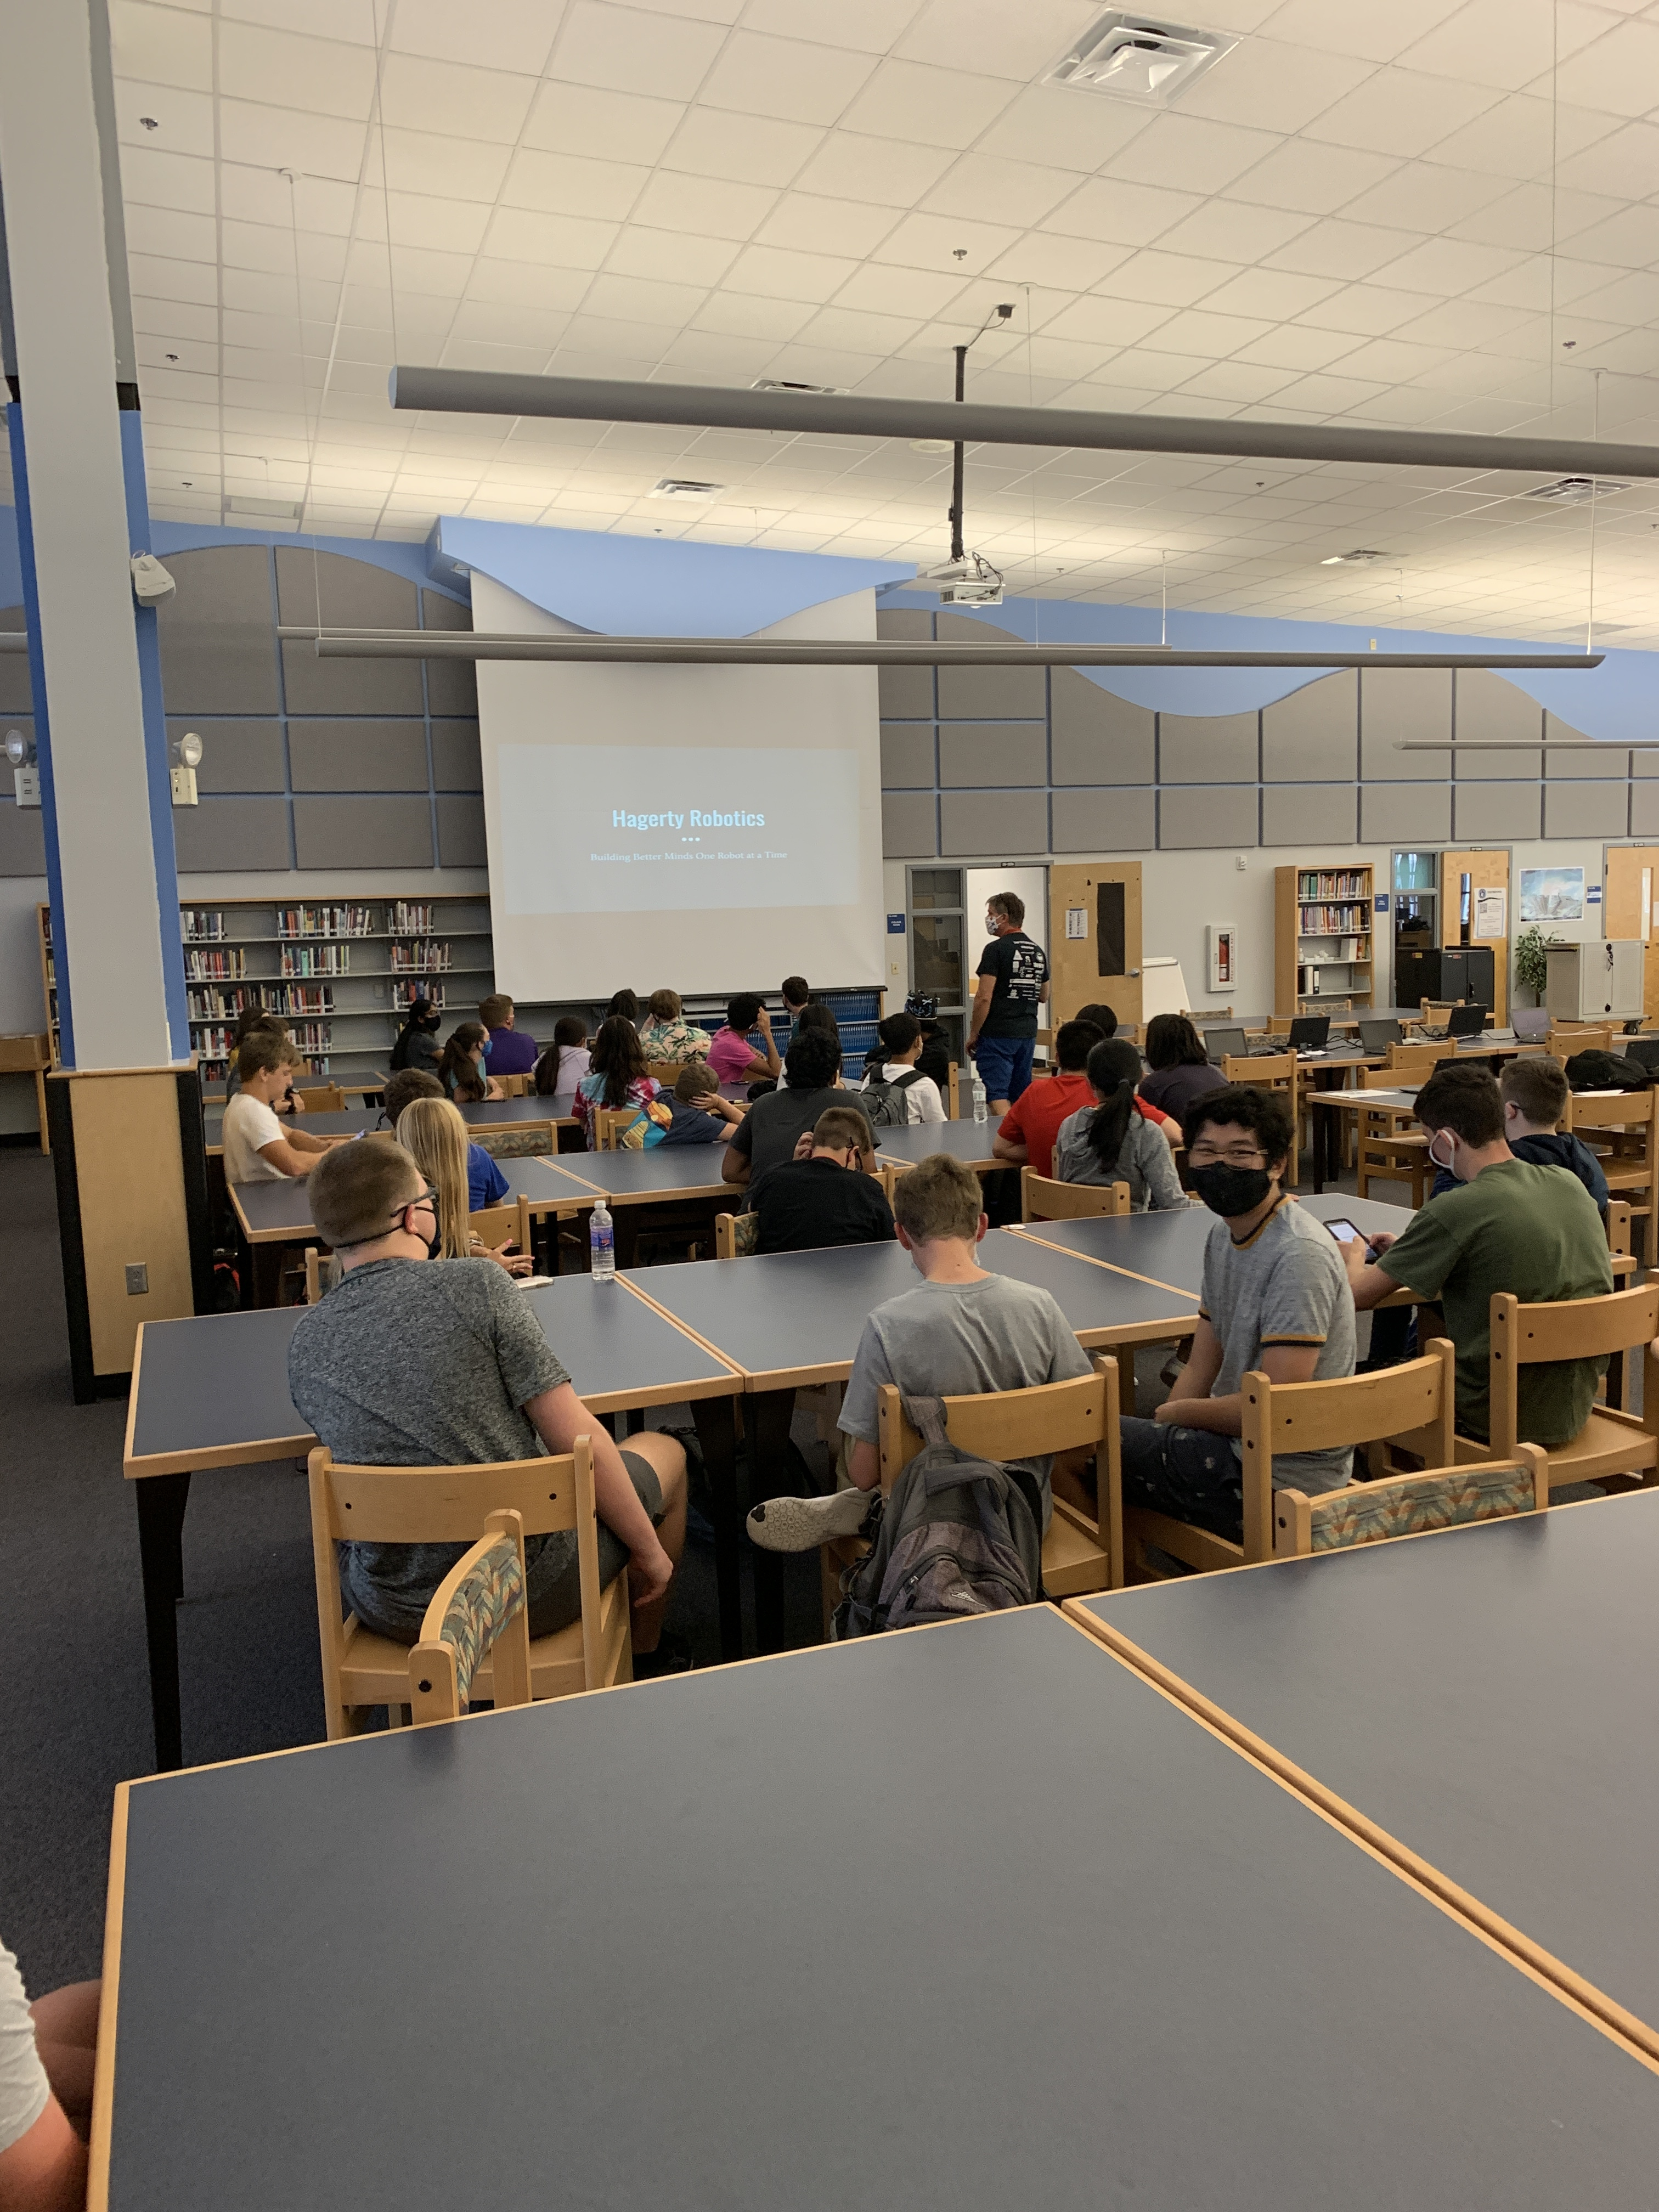
\includegraphics[width=0.95\textwidth]{Meetings/August/08-11-21/IMG_2430 - Nathan Forrer.JPG}
  \caption{Mr. Ibarguen's new member orientation}
  \label{fig:081121_1}
\end{minipage}%
\hfill%
\begin{minipage}[b]{.48\textwidth}
  \centering
  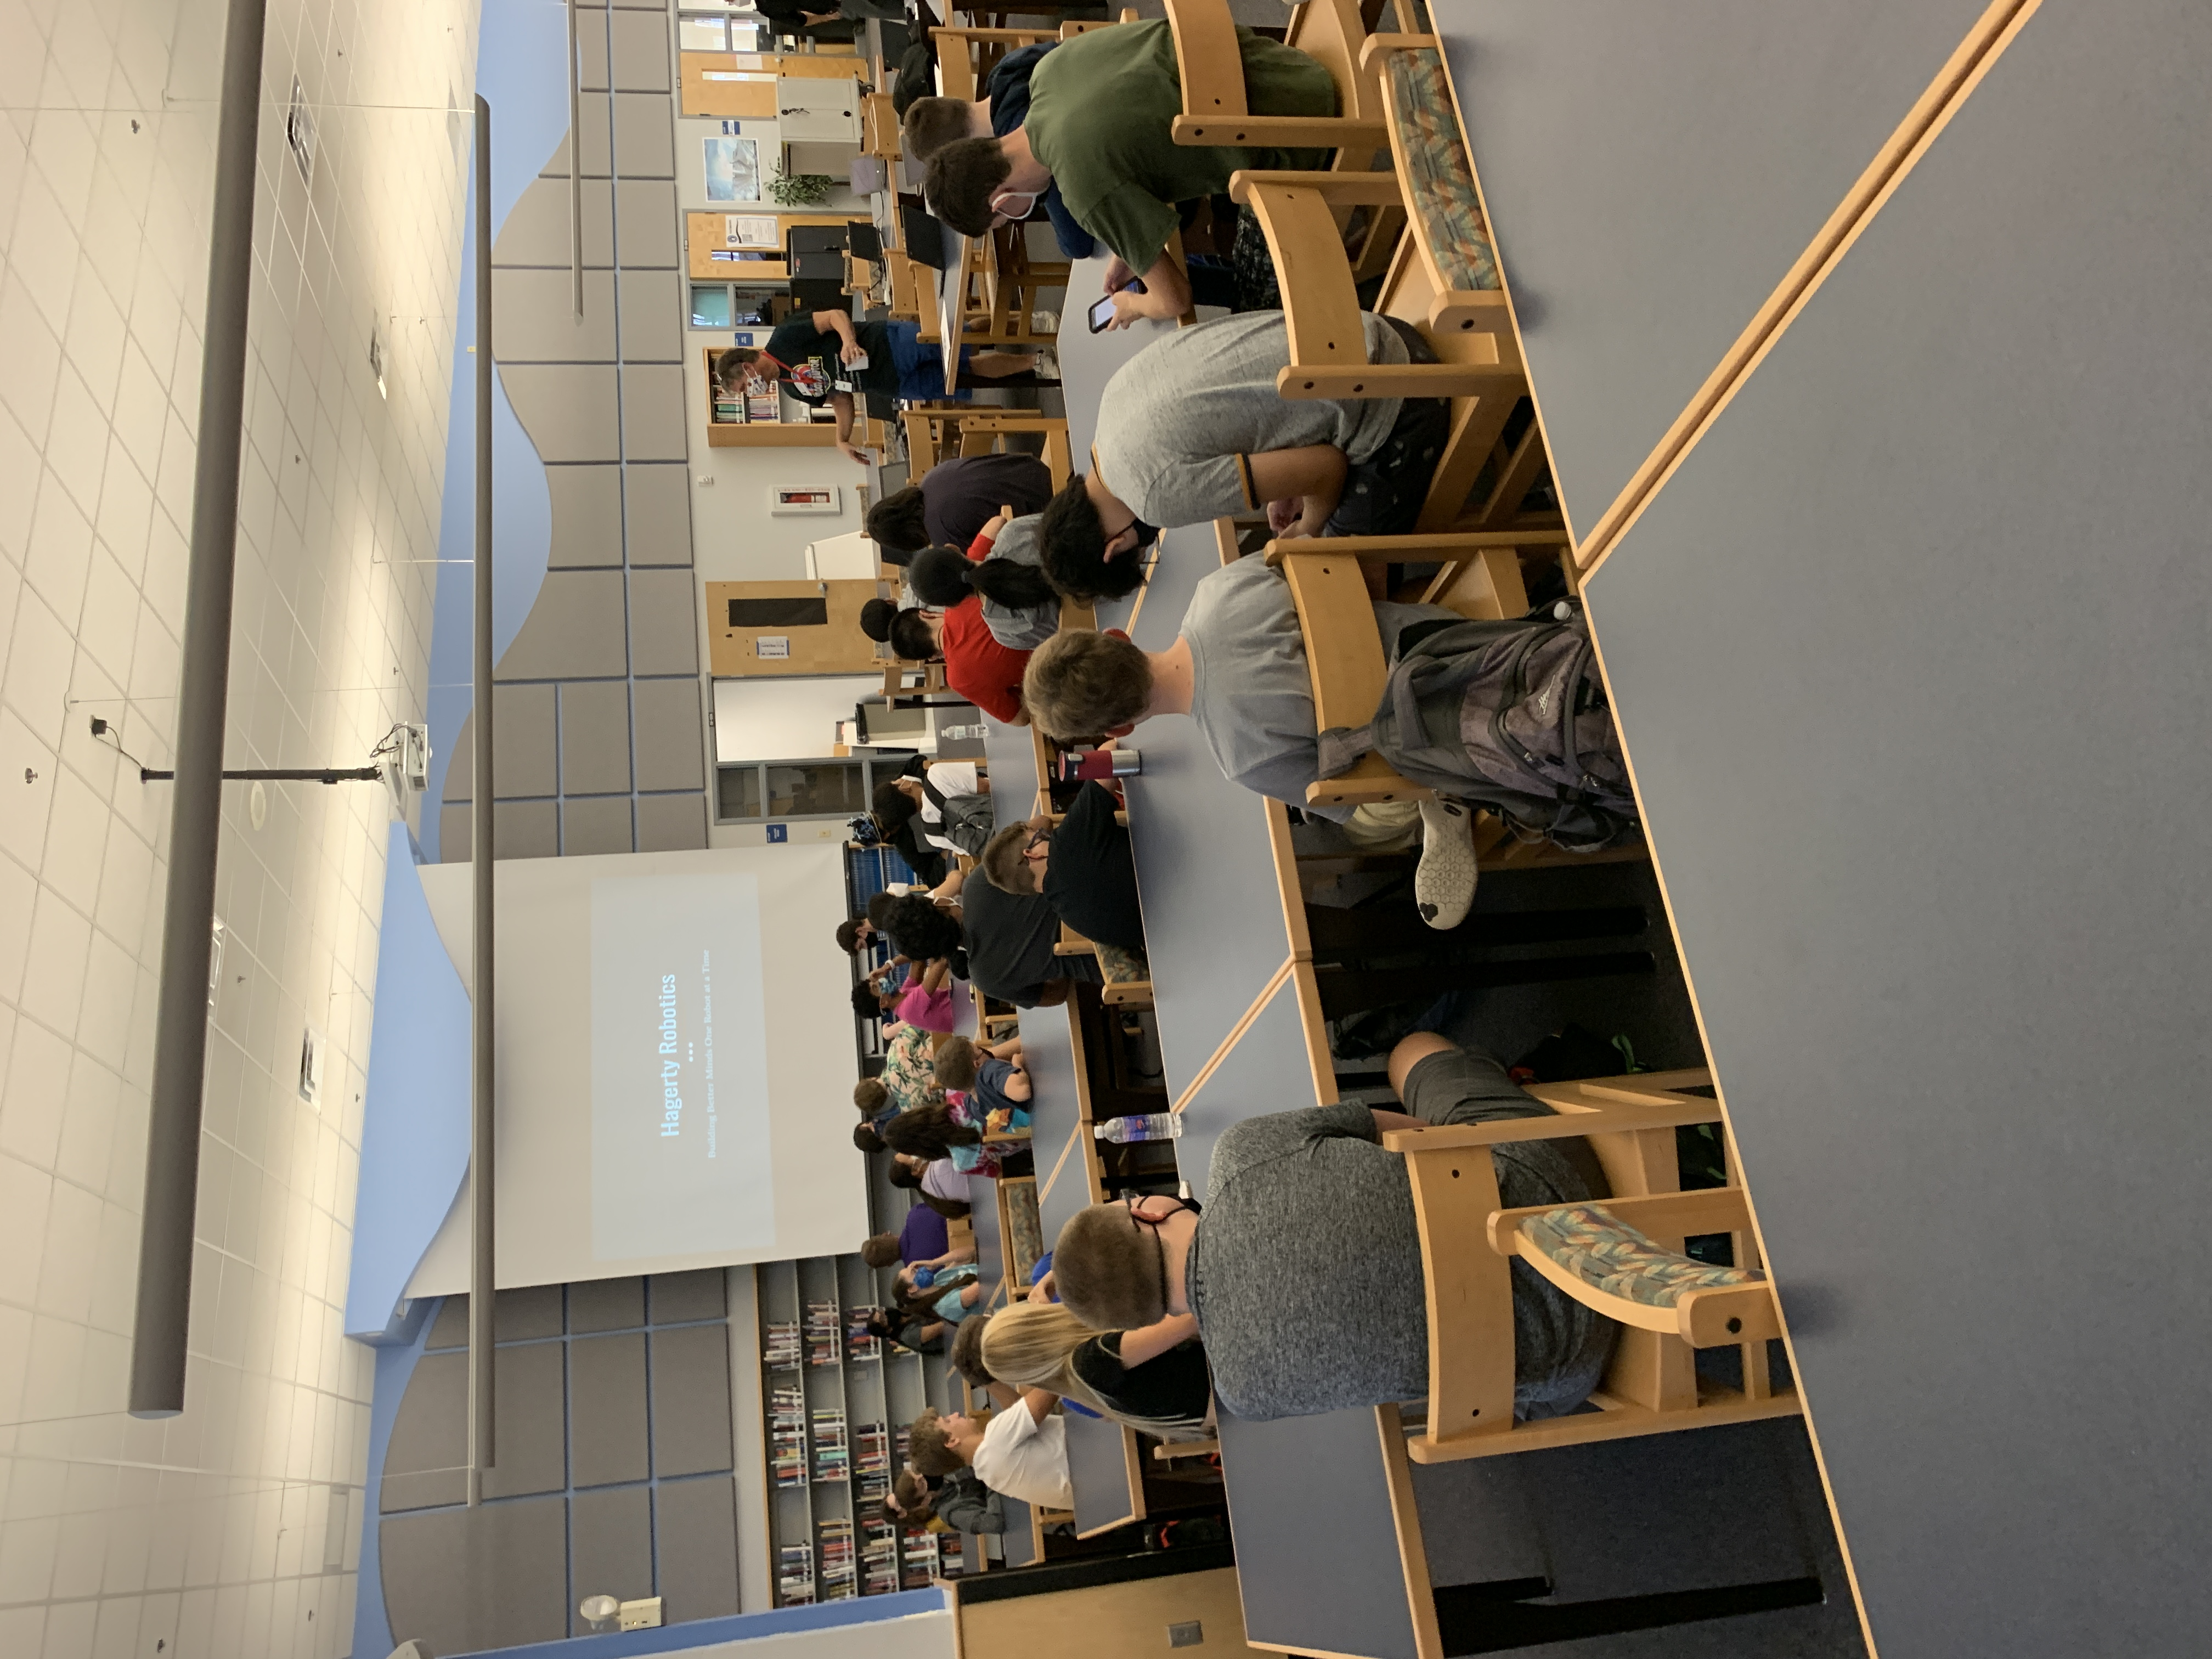
\includegraphics[width=0.95\textwidth]{Meetings/August/08-11-21/IMG_2432 - Nathan Forrer.JPG}
  \caption{More Orientation}
  \label{fig:081121_2}
\end{minipage}
\end{figure}


\whatsnext{
\begin{itemize}
    \item allow new members to choose their preferred team between FIRST and VEX
    \item organize into teams
\end{itemize} 
}

